\documentclass[tikz,border=2pt]{standalone}
\usepackage{amsmath,amssymb}
\usepackage{tikz}
\usetikzlibrary{arrows.meta}

\begin{document}
% Skew lines in R^3: one runs along the floor, the other passes above it in a different
% direction; they are not parallel and never meet.
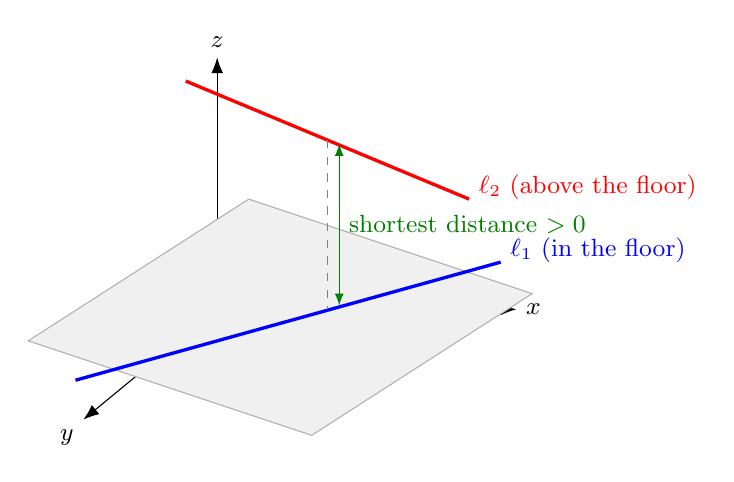
\begin{tikzpicture}[every node/.style={font=\small}, >={Latex[length=2mm]}]
	\draw[->] (0,0) -- (3.8,0) node[right] {$x$};
	\draw[->] (0,0) -- (0,3.2) node[above] {$z$};
	\draw[->] (0,0) -- (-1.7,-1.4) node[below left] {$y$};
	\fill[gray!12] (-2.4,-0.4) -- (1.2,-1.6) -- (4.0,0.2) -- (0.4,1.4) -- cycle;
	\draw[gray!60] (-2.4,-0.4) -- (1.2,-1.6) -- (4.0,0.2) -- (0.4,1.4) -- cycle;
	\draw[blue, very thick] (-1.8,-0.9) -- (3.6,0.6);
	\node[blue, anchor=west] at (3.6,0.75) {$\ell_1$ (in the floor)};
	\draw[red, very thick] (-0.4,2.9) -- (3.2,1.4);
	\node[red, anchor=west] at (3.2,1.55) {$\ell_2$ (above the floor)};
	\draw[dashed, gray] (1.4,2.15) -- (1.4,0.0);
	\draw[{Latex[length=1.5mm]}-{Latex[length=1.5mm]}, green!50!black] (1.55,2.1) -- (1.55,0.05) node[midway, right, font=\small] {shortest distance $>0$};
\end{tikzpicture}
\end{document}
